% !TEX encoding = UTF-8
% !TEX TS-program = pdflatex
% !TEX root = ../tesi.tex

%**************************************************************
\chapter{Descrizione dello stage}
\label{cap:descrizione-stage}
%**************************************************************

Il capitolo riporta una descrizione dettagliata dell'attività di stage svolta, analizzando brevemente i possibili rischi, le problematiche da risolvere e le soluzioni proposte. Sono inoltre riportate la pianificazione del lavoro e i requisiti richiesti prima dell'inizio dello stage. 

%**************************************************************
\section{Analisi dei rischi}

Al fine di evitare rallentamenti dei periodi di lavoro è stata effettuata una breve analisi dei
rischi, in modo da evitare le situazioni che portano alla creazione di eventi non pianificati,
ove possibile. 
I rischi analizzati sono divisi per area di competenza, e per ognuno di essi è mostrata brevemente la strategia di mitigazione dello stesso.

\begin{itemize}
	\item livello tecnologico
	\begin{itemize}
		\item \textbf{Tecnologie sconosciute:} L'utilizzo di tecnologie sconosciute, come i servizi di Microsoft, potrebbero portare a ritardi o a difficoltà nello svolgimento del progetto. Tuttavia, grazie al periodo di apprendimento pianificato nel primo periodo dello stage e grazie alla presenza di programmatori esperti nel settore con cui confrontarsi, questo rischio non dovrebbe presentarsi;
		\item \textbf{Guasti hardware:} Durante lo svolgimento dello stage è possibile che la strumentazione utilizzata, in particolare il computer assegnato, possa incorrere in guasti hardware rischiando rallentamenti e perdita del lavoro. Per scongiurare questo evento, una copia delle soluzioni è salvata regolarmente in una cartella del server dell'azienda destinata allo studente.   
	\end{itemize}
	\item livello organizzativo
	\begin{itemize}
		\item \textbf{Valutazione delle risorse:} Data la poca esperienza con progetti di queste dimensioni si potrebbe incorrere in un'errata valutazione delle risorse, generando sprechi delle stesse o ritardi. Per mitigare questo rischio, ogni settimana avviene un incontro con il tutor aziendale per valutare il lavoro svolto e chiarire dubbi qualora si presentassero.
	\end{itemize}
	\item livello dei requisiti
	\begin{itemize}
		\item \textbf{Incomprensioni e scelte non ottimali:} è possibile che alcuni requisiti siano fraintesi o valutati erroneamente, portando allo sviluppo di un prodotto non consono alle aspettative dell'azienda. Per mitigare questo rischio, ogni settimana avviene un incontro con il tutor aziendale per valutare il lavoro svolto e chiarire dubbi qualora si presentassero.
	\end{itemize}
\end{itemize}

%**************************************************************
\section{Modalità di svolgimento}
L’attività di stage è stata svolta presso la sede dell’azienda per favorire l’interazione dello studente con il tutor e per affacciarlo nella realtà di un team di lavoro aziendale. Lo stagista ha avuto quindi la possibilità di confrontarsi con programmatori più esperti ed essere supportato al meglio in caso di problematiche di sviluppo e gestione del progetto.
Lo studente ha potuto confrontarsi con il tutor per qualsiasi problematica, mentre l’organizzazione settimanale del lavoro è stata gestita tramite dei meeting atti a definire lo stato di avanzamento del progetto e rivedere in tempo reale obiettivi settimanali o miglioramenti del prodotto sulla base dei risultati ottenuti dallo sviluppo.\\ I risultati sono stati valutati settimanalmente (o al termine dell’attività prevista) in base alla quantità e alla qualità dei prodotti forniti dallo studente.
L’orario lavorativo era il seguente: dal lunedì al venerdì dalle 8:40 alle 12:40 e dalle 13:30 alle 17:30.

%**************************************************************
\section{Cos'è una licenza Software}

Una licenza software è il contratto con il quale il titolare dei diritti sul software, di norma il produttore, concede all'utente il diritto di utilizzare il software, secondo i termini e le condizioni stabilite nel contratto stesso.
\\
Ogni installazione di software è accompagnata da una licenza. In un accordo di licenza può essere definito quanti utenti possono utilizzare il Software. Poichè ogni cliente necessita di esigenze diverse, esistono diverse tipologie di licenze del \textit{Software Gestionale Vision}, ognuna delle quali conferisce diverse funzionalità. 
\\
Le licenze software concedono all'utente il diritto d'uso sul prodotto software, sempre nel rispetto delle regole in esse contenute. I clienti in possesso di regolare licenza hanno la certezza di utilizzare il software originale, e rispettando le condizioni d'uso stabilite in fase di acquisto hanno la garanzia di essere conformi alle norme sul diritto d'autore e quindi di non incorrere in nessuna sanzione legale per violazioni della legge.
\\
L'acquisto di una licenza del \textit{Software Gestionale Vision} consiste nel ricevere un \texttt{Product Key}, ovvero una sequenza di 20 caratteri, univoca per ogni licenza, da utilizzare in fase di attivazione. Al \texttt{Product Key} è legato un \texttt{Serial Number}, composto da 6 cifre, e una \texttt{Tipologia}, che specificano quale licenza si ha acquistato e che funzionalità offre.
\\
Per semplicità, nel documento una licenza sarà trattata come l'insieme di \texttt{Product Key}, \texttt{Serial Number}, \texttt{Tipologia} e tutte le caratteristiche che la compongono, come la data di attivazione o il cliente a cui è stata venduta.

%**************************************************************
\newpage
\section{Problematiche da affrontare}
Nella presente sezione sono analizzate le problematiche da risolvere attraverso l'attività di stage. La descrizione delle problematiche è quindi da contestualizzarsi nel periodo antecedente lo stage.

\subsection{Creazione di una licenza}

La creazione di una nuova licenza avviene tramite il Software \textit{GenPK}. Esso offre la possibilità di creare uno o più \texttt{Product Key} a partire da \texttt{Serial Number} e \texttt{Tipologia} della licenza.
Il \texttt{Serial Number} può essere creato nei seguenti modi:
\begin{itemize}
\item \textbf{Manuale:} Sono utilizzate sei cifre scelte liberamente dal creatore. Se il numero scelto è già in uso è segnalato un errore;
\item \textbf{Casuale:} È fornito un numero a sei cifre casuale. Se il numero generato è già in uso è segnalato un errore; 
\item \textbf{Prime due cifre per l'anno:} Le prime due cifre corrispondono alle ultime due cifre dell'anno in corso, per tenere traccia dell'anno in cui il \texttt{Product Key} è stato generato. Al creatore è data la possibilità di scegliere il valore delle restanti quattro cifre, da cui partirà la ricerca per il primo \texttt{Serial Number} libero.
\end{itemize}
La \texttt{Tipologia} è scelta tra una delle seguenti:
\begin{itemize}
\item \textbf{LT}: gestionale semplice per le piccole aziende;
\item \textbf{ERP}: gestionale completo per le piccole e medie imprese;
\item \textbf{SQL:} estensione di ERP, con funzionalità ancora maggiori;
\item \textbf{Trasporti:} gestionale dedicato alle aziende di trasporto merci e persone, in particolare alla gestione dei carichi completi.
\end{itemize}

I product key creati sono salvati all'interno di un file, contenente la totalità dei dati delle licenze, con lo stato della licenza impostato a "da attivare". Il file delle licenze è scaricato all'avvio di \textit{GenPK} tramite server (GLOSSARIO)FTP aziendale ed è rinviato al server alla chiusura del programma. Lo scambio del file tramite protocollo FTP e l'avere il file a disposizione, seppur in modo riservato, sul proprio PC durante l'operazione espone l'intero sistema ad alti rischi come la corruzione del file con conseguente perdita di dati o la contraffazione degli stessi.\\
Infine, poiché i dati sono salvati su un unico file, per preservare la consistenza dei dati non è possibile avviare \textit{GenPK} su più macchine contemporaneamente.

\subsection{Attivazione di una licenza} 
Il cliente al primo avvio del \textit{Software Gestionale Vision} è invitato a inserire il \texttt{Product Key} ricevuto in fase d'acquisto. Il Software verifica che lo stato del \texttt{Product Key} sia impostato su "da attivare", preleva il (GLOSSARIO)MAC Address della scheda di rete su cui sta avvenendo l'installazione e, insieme al \texttt{Product Key}, attraverso un algoritmo di cifratura crea l’\texttt{Activation Key}, una stringa che sarà utilizzata per verificare che la licenza sia in uso sulla stessa macchina su cui è stata attivata. Lo stato del \texttt{Product Key}, dopo l'attivazione, viene modificato da “da attivare” ad “attivato”. Come nella creazione della licenza, i cambi di stato e la lista dei Product Key sono contenute in un file che il Software scarica sul PC in uso tramite protocollo FTP dal server dell’azienda, rinviato al server una volta modificato. Questa procedura, com'è già stato evidenziato nel paragrafo precedente, è molto rischiosa, poiché tutte le licenze sono disponibili su un file che potrebbe essere facilmente corrotto o manomesso.\\
Un esempio di attacco tramite questo sistema è poter usufruire di infinite licenze acquistandone due. 
Il meccanismo dell'attacco è semplice, ed è illustrato nei seguenti passaggi:
\begin{enumerate}
\item l'utente malevolo attiva il primo \texttt{Product Key} su una macchina. Lo stato del \texttt{Product Key} viene impostato correttamente da "da attivare" ad "attivato"; 
\item l'utente procede con l'attivazione del secondo \texttt{Product Key}, ma prima di terminare l'operazione il file contenente i dati delle licenze viene modificato, impostando lo stato del primo \texttt{Product Key} a "da attivare";
\item il primo \texttt{Product Key} è quindi disponibile per una nuova installazione.
\end{enumerate}
Questo tipo di attacco è permesso per due motivi. In primo luogo il file contenente i dati delle licenze è salvato sul PC dell'utilizzatore. Anche se cifrato non è difficile capire le stringhe corrispondenti ai termini "da attivare" e "attivato", ed è quindi possibile modificarlo senza conoscere il metodo di cifratura. In secondo luogo i controlli di validità della licenza, come il verificare che la licenza sia attiva su un solo PC per volta, sono svolti totalmente in locale. Quindi, potendo reinstallare il Software su una nuova macchina (ricreando quindi i dati per il controllo), i controlli saranno sempre superati, perché il sistema non ha modo di capire che la licenza è stata installata due volte, ma capirebbe solo se l'installazione del programma sarebbe copiata su un'altra macchina. 

\subsection{Avvio del Software Gestionale Vision} 

All'avvio del \textit{Software Gestionale Vision} è letta una chiave di registro contenente il \texttt{Product Key} della licenza, è prelevato il MAC Address della scheda di rete e insieme, con lo stesso algoritmo di cifratura utilizzato in fase di attivazione, è creato l'\texttt{Activation Key}. Il codice appena creato è controllato con l’Activation Key salvata in fase di attivazione in una chiave di registro; se è uguale allora la macchina utilizzata per accedere è la stessa su cui è stato installato il \textit{Software Gestionale Vision}, e l’utente può utilizzare il programma normalmente.\\
Poiché il controllo è svolto totalmente in locale esso è facilmente aggirabile attraverso l’uso di macchine virtuali identiche. Infatti, installando il \textit{Software Gestionale Vision} in una macchina virtuale e clonando quest'ultima, il controllo Hardware avrebbe sempre successo, potendo utilizzare di fatto una licenza su un numero illimitato di macchine. 
\\Un'altra problematica sorge da un qualsiasi guasto, o al cambio, della scheda di rete in quanto il controllo Hardware fallirebbe, e il cliente sarebbe costretto a contattare l’azienda per risolvere la situazione poiché l'\texttt{Activation Key} risultante sarebbe diversa, il che blocca l'esecuzione del Software.

\subsection{Caricamento dei moduli di una licenza} 
Il caricamento dei moduli di una licenza, ossia quali funzioni sono permesse, avviene da un file in formato “.HWK”, generato per mezzo del 
programma \textit{GenFileKey}, inviato ai clienti e salvato nella cartella del Software Gestionale Vision. Esso contiene un codice cifrato, visibile all’utente, riepilogativo dei moduli attivi della licenza. Questo file può essere aperto con qualsiasi editor di testo e facilmente modificato, rischiando di compromettere la licenza.

\subsection{Licenze bloccate} 

Le licenze bloccate dall'azienda sono contenute in una Blacklist salvata all’interno del Software Gestionale Vision. Qualora l'azienda volesse aggiungere una nuova licenza nella Blacklist dovrebbe rilasciare un aggiornamento del proprio Software per far si che il programma riconosca la nuova licenza bloccata e non si avvii.
\\Questo provoca che un utente, non aggiornando il proprio programma (il che è consentito), può continuare a utilizzare il \textit{Software Gestionale Vision} anche in caso di licenza bloccata. 

\subsection{Procedura di disattivazione} 
Per disattivare la licenza dal proprio computer e reinstallarla in un altro il cliente è sempre costretto a contattare l'azienda. Questo provoca sia un onere non indifferente per l'azienda, soprattutto nei casi di rinnovamento delle macchine di un'azienda cliente, sia una condizione non ottimale da parte del cliente che si trova costretto a contattare l'azienda quando potrebbe acquisire autonomia con il click di un semplice pulsante.

\subsection{Scadenza di una licenza} 
Le licenze non possiedono una data di scadenza. L'acquisto avviene sottoscrivendo un contratto per l'utilizzo del Software e per disporre dell'assistenza tecnica, quindi un utente acquistando il Software una singola volta potrà sempre utilizzarlo. Solo in caso di nuovi aggiornamenti il cliente potrebbe voler riacquistare il Software, ma questo non è assolutamente necessario. 
\\Questa politica genera uno scarso controllo sullo stato delle licenze vendute, e inoltre limita i profitti dell'azienda. Vendere una licenza per un periodo definito piuttosto che per un tempo illimitato è una strategia molto utilizzata, accettata dai clienti e fornisce margini di guadagno molto migliori.

\subsection{Rivenditori} 
L'azienda \textit{VISIONEIMPRESA} oltre ai clienti finali gestisce dei rivenditori in grado di vendere il \textit{Software Gestionale Vision} a terzi. 
I rivenditori per operare, ad esempio per creare una licenza o gestirne i moduli, devono sempre contattare l'azienda, in modo che essa sia sempre aggiornata sulla situazione delle proprie licenze e che possa fatturare quanto venduto. I rivenditori quindi dispongono di un'autonomia molto limitata, generando situazioni poco confortevoli e oneri non necessari.

\subsection{Monitoraggio delle licenze}
L'azienda può monitorare lo stato delle licenze attraverso il Software \textit{GenPK}, ma le informazioni da esso mostrate sono minime, come il cliente associato e la tipologia, o il numero di licenze vendute per tipologia. Altre informazioni fondamentali, come i moduli di una licenza, non sono facilmente reperibili, e avere una visione completa, comprendente anche i rivenditori, aiuterebbe sicuramente ad ottenere una migliore gestione.



%**************************************************************
\section{Soluzioni proposte}

In relazioni alle problematiche analizzate nel precedente paragrafo, sono proposte le seguenti soluzioni. In questa sezione le soluzioni proposte sono trattate sommariamente, per lasciare una definizione completa delle stesse nelle sezioni {\hyperref[cap:sviluppo-software]{Web Service e Database}}, {\hyperref[cap:license-manager]{License Manager 1.0}} e {\hyperref[cap:moduli-vision]{Moduli Software Gestionale Vision}}.

\subsection{Creazione di una licenza}

La creazione delle licenze avviene tramite il Software \textit{License Manager 1.0}, in sostituzione del Software \textit{GenPK}. Il Software riprende le modalità di creazione di \textit{GenPK}, ma elimina il sistema del file contenente i dati delle licenze ottenuto tramite FTP, e si occupa di salvare le licenze create in un Database. Le operazioni di generazione e salvataggio della  licenza sono gestiti tramite Web Service. 
Il passare da un file condiviso (perennemente a rischio per via dei salvataggi sui PC degli utenti) a un sistema che utilizza un Database per archiviare e ottenere i dati aumenta di molto la sicurezza della gestione delle licenze.

\subsection{Attivazione di una licenza}

L'attivazione di una licenza richiede come nella precedente procedura l'inserimento del \texttt{Product Key} ricevuto in fase d'acquisto, e in seguito, tramite Web Service, è controllato che esso sia disponibile per un'installazione. Le modifiche di stato avvengono nel Database, eliminando di fatto l'utilità del file condiviso tramite FTP e riducendo la possibilità di attacchi. L’\texttt{Activation Key}, utilizzata per il controllo Hardware, è eliminata e rimpiazzata da un nuovo sistema. Il controllo Hardware è ora basato su un insieme di componenti e non solo sul \texttt{MAC Address} della scheda di rete, in modo da permettere all’utente di cambiare alcune delle componenti del pc (ad esempio in caso di guasti) e non dover ricontattare l’azienda per poter continuare a utilizzare il \textit{Software Gestionale Vision}. 
Infine, nella prima attivazione il cliente dovrà associare un indirizzo email alla propria licenza, in modo che possa disattivare e reinstallare il programma senza il bisogno di dover contattare l’azienda. Associando un indirizzo email l'utente sarà in grado di riutilizzare autonomamente la propria licenza nella reinstallazione del Software, anche qualora sia impossibilitato a disattivarla, come nel caso di guasto o reinstallazione del sistema operativo del PC in cui la licenza era utilizzata.


\subsection{Avvio del Software Gestionale Vision}

Come analizzato nelle problematiche, l'unico controllo di validità della licenza all'avvio del Software avveniva in locale, controllando l'\texttt{Activation Key}, ma permettendo di fatto di utilizzare la licenza per un periodo illimitato e in più macchine virtuali grazie alla clonazione. Nel sistema attuale sono stati implementati due  diversi controlli, uno per un accesso senza connessione a Internet e uno per l’accesso con connessione.
\\
Il controllo per l’avvio del Software in Offline utilizza informazioni salvate in chiavi di registro per verificare la validità della licenza. È stato realizzato anche un metodo basato sulle firme digitali per verificare l’integrità delle chiavi di registro, così che non possano essere manomesse facilmente. L’utilizzo del programma in Offline è ora permesso per 15 giorni, scaduti i quali sarà chiesto di connettersi a internet.
\\
Il controllo all'avvio Online è formato da due procedure:
\begin{itemize}
\item all'avvio, tramite Web Service, è controllata la licenza in termini di data di scadenza, bloccaggio e componente Hardware;
\item a intervalli di un'ora (tempo riducibile nell'effettiva implementazione del modulo a discrezione dei programmatori) è controllato che l'utente non stia utilizzando il programma su macchine differenti ma con stesso Hardware (ad esempio in seguito a una clonazione di una macchina virtuale).

\end{itemize}

\subsection{Caricamento dei moduli della licenza}

Il codice cifrato riepilogativo dei moduli è ora salvato in un Database, eliminando la necessità di inviare un file ai clienti e la possibilità che esso venga corrotto. La generazione del codice che prima avveniva tramite il Software \textit{GenFileKey} ora è eseguita da \textit{License Manager 1.0}.

\subsection{Licenze bloccate} 
Il controllo di una licenza bloccata, disponendo di un Database cui il \textit{Software Gestionale Vision} si riferisce per ritirare i dati, è ora immediatamente implementabile controllando il campo dedicato relativo alla licenza ispezionata. L'utente quindi non potrà più utilizzare una licenza bloccata evitando di aggiornare il \textit{Software Gestionale Vision}, e l'azienda non dovrà rilasciare un nuovo aggiornamento per inserire una licenza bloccata nella Blacklist.
Il blocco è eseguito tramite una funzionalità di \textit{License Manager 1.0}.

\subsection{Procedura di disattivazione}

Grazie all'associazione di un indirizzo email alla propria licenza un utente è ora in grado di disattivare e reinstallare in sicurezza la propria licenza ogni volta che lo desidera, senza dover contattare l’azienda e in qualsiasi situazione. La disattivazione può comunque essere gestita dall'azienda tramite \textit{License Manager 1.0}.

\subsection{Scadenza di una licenza}

Nel nuovo sistema di gestione e controllo delle licenze è stata implementata la data di scadenza, permettendo all'azienda di avere un controllo maggiore sulle proprie licenze e poter modificare il metodo di vendita. È implementato un controllo sulla data di scadenza sia all'avvio in Offline sia in Online. Nel controllo all’avvio del programma è anche controllato che la licenza non sia entrata nell’ultimo mese di validità. In quel caso sarà mostrato un GLOSSARIO \textit{reminder} con i giorni rimanenti prima della scadenza. 
 
\subsection{Rivenditori}

\textit{License Manager 1.0}, grazie al suo sistema di utenti, può essere distribuito ai rivenditori identificandoli con utenti di tipo \texttt{Guest}, lasciando loro un certo grado di libertà che non li costringa a rivolgersi all’azienda per ogni decisione. Ogni azione da loro intrapresa è comunicata all’azienda tramite email, e tutti gli stati precedenti alle modifiche sono registrati in una tabella dedicata del Database. La comunicazione all'azienda delle modifiche apportate dai rivenditori è fondamentale perché l'azienda sia sempre aggiornata sullo stato delle proprie licenze.

\subsection{Monitoraggio delle licenze}

\textit{License Manager 1.0} fornisce un sistema di monitoraggio migliore, basato su:
\begin{itemize}
\item visione completa di tutte le caratteristiche di una licenza (ad esempio la data di scadenza, le componenti Hardware associate o i moduli definiti);
\item statistiche sulla distribuzione e l'utilizzo delle licenze, filtrabili anche per i rivenditori;
\item log degli accessi al \textit{Software Gestionale Vision} per notare possibili anomalie.
\end{itemize}
Grazie al nuovo sistema di monitoraggio l'azienda può visualizzare in ogni momento la situazione delle sue licenze, e avere statistiche per apportare miglioramenti al proprio Software.


%**************************************************************
\newpage
\section{Pianificazione del Lavoro}

La seguente sezione mostra la pianificazione del lavoro attuata prima di iniziare l'attività di stage e l'effettivo utilizzo delle ore. Per rendere più chiara la pianificazione del lavoro e lo svolgimento effettivo delle attività sono utilizzati Diagrammi di Gantt.
\newpage

\subsection{Pianificazione antecedente lo stage}
Nella Figura \ref{primastage} è mostrata la pianificazione dello stage prima di iniziare l'attività. La figura è disposta verticalmente per aumentare la visibilità.
\\
\\

\rotatebox{90}{\begin{minipage}{0.85\textheight}
%\begin{figure}
\centering
    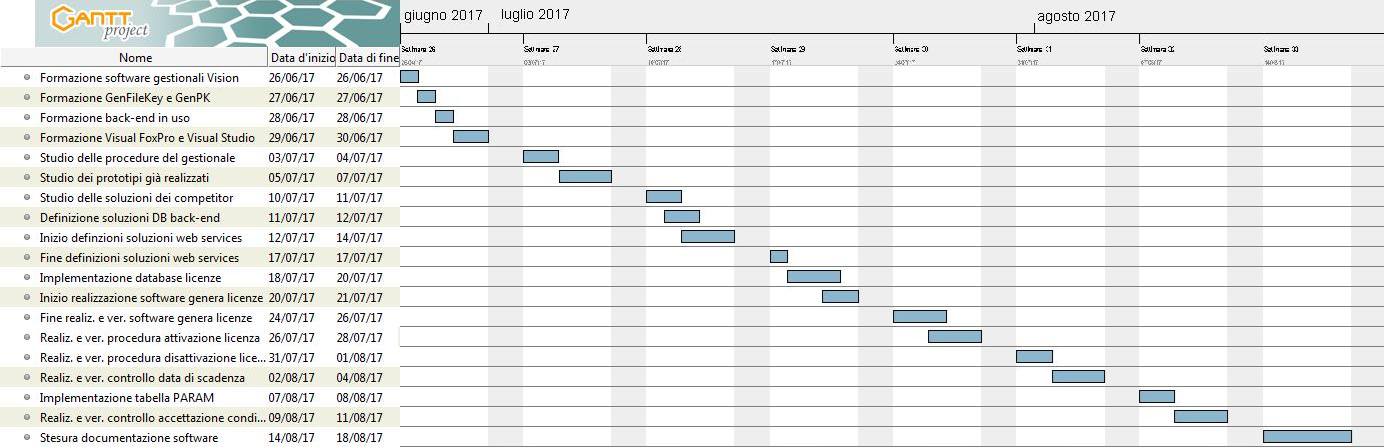
\includegraphics[width=\textwidth]{ganttPrima} 
    \captionof{figure}{Diagramma di Gantt - Pianificazione del lavoro}
    \label{primastage}
    \end{minipage}}
%\end{figure}
\newpage

\subsection{Resoconto delle attività svolte}
Nella Figura \ref{dopostage} è mostrata la suddivisione delle attività effettivamente svolte. Essa si discosta di molto rispetto quanto pianificato prima di iniziare lo stage. Infatti, grazie a un veloce apprendimento e a una buona progettazione, è stato possibile organizzare il tempo a disposizione per realizzare anche gli obiettivi secondari e facoltativi.
\\
\\
\rotatebox{90}{\begin{minipage}{0.85\textheight}
%\begin{figure}
\centering
    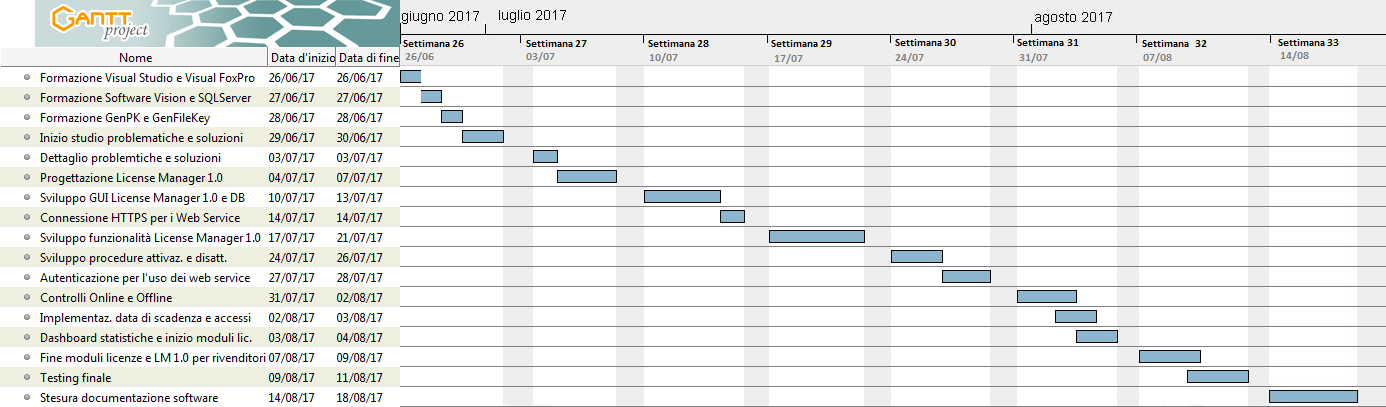
\includegraphics[width=\textwidth]{effettivostage} 
    \captionof{figure}{Diagramma di Gantt - Attività svolte}
    \label{dopostage}
    \end{minipage}}
%\end{figure}
\newpage

%**************************************************************
\section{Obiettivi e Requisiti}

\subsection{Obiettivi}
Nella fase preliminare dello stage sono stati delineati i seguenti obiettivi, in ordine di importanza. Gli obiettivi sono identificati da un codice così composto:
$$ XXYY $$

dove XX rappresenta la tipologia dell'obiettivo e YY è un numero progressivo utilizzato per differenziare gli obiettivi della stessa categoria.
\\
Le sigle utilizzate sono le seguenti:

\begin{itemize}
\item \textbf{OP:} obiettivo primario;
\item \textbf{OS:} obiettivo secondario;
\item \textbf{OF:} obiettivo facoltativo;
\item \textbf{FO:} obiettivo formativo.
\end{itemize}

Gli obiettivi identificati sono così suddivisi:

\begin{itemize}

\item \textbf{obiettivi primari:}\begin{itemize}
\item OP01: definizione delle strategie risolutive per le problematiche presentate;
\item OP02: implementazione di un sistema di attivazione e disattivazione delle licenze via web services;
\item OP03: implementazione di controlli per la validità di una licenza.
\end{itemize}
\item \textbf{obiettivi secondari:}\begin{itemize}
\item OS1: implementazione della data di scadenza di una licenza e relativi controlli.
\end{itemize}
\item \textbf{obiettivi facoltativi:}\begin{itemize}
\item OF01: implementazione delle licenze per moduli;
\item OF02: raccolta dei dati sull’attivazione delle licenze e sul loro utilizzo;
\item OF03: creazione di una dashboard con statistiche e alert sulle licenze in uso, disattivate, e anomalie.
\end{itemize}
\item \textbf{obiettivi formativi:}\begin{itemize}
\item FO01: acquisizione di competenze utili allo sviluppo di software gestionale;
\item FO02: interazione con un team di lavoro aziendale;
\item FO03: ottenimento di capacità decisionali sulle migliori tecnologie da utilizzare in diversi contesti.
\end{itemize}

\end{itemize}

Durante lo svolgimento dello stage, oltre alla creazione e all'attivazione di una licenza, è stato deciso di sviluppare il Software \textit{License Manager 1.0} per gestirne tutti gli aspetti. Dopo aver raggiunto tutti gli obiettivi prefissati, è stato posto come obiettivo ultimo la distribuzione del Software \textit{License Manager 1.0} anche ai rivenditori dell'azienda per concedere loro un certo grado di libertà nella creazione e nella modifica delle licenze. 

\subsection{Requisiti}

In relazione agli obiettivi presentati nel paragrafo precedente, sono stati identificati i requisiti riportati in seguito.

\subsubsection{Requisiti OP01}
Per definire una valida strategia risolutiva per le problematiche presentate sono stati identificati i seguenti requisiti:

\begin{itemize}
\item deve essere svolta un'analisi dettagliata del sistema di gestione delle licenze in uso, per analizzarne criticità e debolezze;
\item deve essere affrontato un periodo di formazione sulle tecnologie da utilizzare, per comprenderne al meglio le potenzialità;
\item devono essere delineate, e approvate dal tutor aziendale, delle soluzioni in grado di risolvere tutte le problematiche presentate.

\end{itemize}

\subsubsection{Requisiti OP02} 
Per implementare un efficiente sistema di attivazione sono stati identificati i seguenti requisiti:
\begin{itemize}
\item deve essere possibile creare un \texttt{Product Key}, secondo le modalità già in uso, da salvare in un Database, eliminando il sistema del file contenente i dati delle licenze, condiviso tramite FTP;
\item l'utente finale deve poter inserire all'avvio del \textit{Software Gestionale Vision} il \texttt{Product Key}, ricevuto in fase d'acquisto, relativo alla licenza per lui creata;
\item il \texttt{Product Key} inserito deve essere controllato tramite un metodo di un Web Service, che provvederà a verificare la disponibilità dello stesso e a impostare le informazioni di attivazione della licenza nella tabella \texttt{Licenze} del database \texttt{DBLicenze};
\item il modulo di attivazione, alla risposta del Web Method, deve impostare le chiavi di registro necessarie per il controllo della licenza in modalità Offline;
\item il modulo di attivazione deve essere in grado di riconoscere se la licenza che si sta attivando è già attiva in un altro computer. In caso positivo, tramite la verifica via email, può disattivarla per attivarla sulla macchina corrente;
\item il modulo di attivazione deve essere in grado di riconoscere se la licenza che si sta attivando è attualmente attiva sul computer corrente, riconoscendo le componenti Hardware ma non trovando i riferimenti dell'attivazione della licenza. In caso positivo, tramite la verifica via email, può procedere con la riattivazione;
\item il modulo di attivazione deve essere in grado di bloccare l'attivazione di una licenza in caso di anomalie (ad esempio se una licenza è bloccata);

\end{itemize} 

Per implementare un efficiente sistema di disattivazione sono stati identificati i seguenti requisiti:


\begin{itemize}
\item il modulo di disattivazione deve leggere le chiavi di registro contenenti i riferimenti della licenza, per sapere quale licenza si vuole disattivare;
\item il modulo deve verificare che l'utente sia autorizzato a disattivare la licenza tramite il controllo via email;
\item il modulo deve procedere con la disattivazione invocando un metodo di un Web Service.
\end{itemize}

\subsubsection{Requisiti OP03}

Per implementare un efficiente sistema di controllo della validità di una licenza sono stati identificati i seguenti requisiti:

\begin{itemize}
\item deve essere implementato un controllo, all'avvio del \textit{Software Gestionale Vision} in modalità Online, per verificare che la licenza sia valida in termini di data di scadenza, bloccaggio e componenti Hardware. Il controllo deve essere eseguito tramite Web Service; 
\item deve essere implementato un controllo, all'avvio del \textit{Software Gestionale Vision} in modalità Offline, per verificare che la licenza sia valida in termini di data di scadenza, bloccaggio e componenti Hardware. Il controllo deve essere svolto in locale tramite l'utilizzo di chiavi di registro;
\item deve essere implementato un controllo, che si ripete durante l'esecuzione del \textit{Software Gestionale Vision}, per verificare che la licenza sia in uso su una solo computer per volta, anche in caso di computer identici come macchine virtuali clonate. Il controllo eve essere eseguito tramite Web Service.
\end{itemize}

\subsubsection{Requisiti OS01}

Per correlare a una licenza la data di scadenza, con i relativi controlli, sono stati identificati i seguenti requisiti:

\begin{itemize}
\item tra i campi di un record licenza, salvato nel Database, deve essere presente la data di scadenza;
\item il Software di gestione delle licenze deve essere in grado di impostare e modificare la data di scadenza di una licenza;
\item all'avvio del \textit{Software Gestionale Vision}, sia in modalità Online che Offline, deve essere controllato che la licenza non sia scaduta;
\item all'avvio del \textit{Software Gestionale Vision}, se la licenza è nell'ultimo mese di scadenza il cliente viene avvisato, per dargli la possibilità di estendere la validità.
\end{itemize}

\subsubsection{Requisiti OF01}

Per implementare efficacemente la gestione dei moduli di una licenza sono stati identificati i seguenti requisti:

\begin{itemize}
\item il Software di gestione delle licenze, \textit{License Manager 1.0}, deve dare la possibilità di scegliere e impostare i moduli di una licenza per ogni tipologia;
\item il codice cifrato riepilogativo dei moduli di una licenza deve essere generato come in \textit{GenFileKey}, per assicurare la compatibilità della soluzione;
\item il codice generato deve essere salvato all'interno di un Database, per evitare che sia disponibile all'utente, riducendo i rischi di sicurezza.

\end{itemize}

\subsubsection{Requisiti OF02}

Per raccogliere dati sull'attivazione delle licenze e sul loro utilizzo sono stati identificati i seguenti requisiti:

\begin{itemize}
\item \textit{License Manager 1.0} deve mostrare all'utente il numero di licenze attivate per tipologia;
\item \textit{License Manager 1.0} deve mostrare all'utente il numero di licenze attivate negli ultimi tre anni;
\item \textit{License Manager 1.0} deve permettere agli utenti Admin di visualizzare i dati sulle attivazioni anche in relazione ai rivenditori.
\end{itemize}


\subsubsection{Requisiti OF03}

Per implementare una dashboard con statistiche e alert sulle licenze in uso sono stati identificati i seguenti requisiti:

\begin{itemize}

\item \textit{License Manager 1.0} deve mostrare statistiche utili, come il numero di licenze bloccate, disattivate, scadute o in scadenza;
\item il modulo di avvio del \textit{Software Gestionale Vision} deve tener traccia degli accessi di un utente, registrando i dati in un apposita tabella del Database. \textit{License Manager 1.0} deve mostrare tali accessi;
\item gli accessi multipli di una licenza, ad esempio da diversi IP o da diversi MAC Address, devono essere evidenziati da \textit{License Manager 1.0}.

\end{itemize}
\subsubsection{Requisiti FO01}

Per acquisire competenzi utili allo sviluppo di Software gestionale sono stati identificati i seguenti requisiti:

\begin{itemize}
\item è necessario intraprendere un periodo di formazione riguardo il \textit{Software Gestionale Vision};
\item è necessario intraprendere un periodo di formazione riguardo i Software di ausilio al \textit{Software Gestionale Vision}, come \textit{GenPK} e \textit{GenFileKey};
\item è necessario analizzare alcune soluzioni sviluppate dai programmatori dell'azienda in contesti simili.
\end{itemize}

\subsubsection{Requisiti FO02}

Per interagire al meglio con il team di lavoro sono stati identificati i seguenti requisiti:

\begin{itemize}
\item è necessario cercare autonomamente possibili soluzioni prima di chiedere aiuto riguardo qualsiasi problematica;
\item è necessario interrogare il team per decisioni importanti o che potrebbero compromettere le funzionalità di un sistema già in uso;
\item è importante saper valutare la frequenza con cui chiedere aiuto, sia per non disturbare il lavoro altrui sia per non rallentare troppo il proprio.
\end{itemize}

\subsubsection{Requisiti FO03}

Per ottenere capacità decisionali sulle tecnologie da utilizzare in diversi contesti sono stati identificati i seguenti requisiti:

\begin{itemize}
\item è necessario approfondire le possibilità di più tecnologie prima di scegliere quale utilizzare;
\item è necessario effettuare dei test per verificare sommariamente che quanto progettato sia effettivamente realizzabile;
\item è necessario attingere informazioni da più fonti per avere una vista più ampia su quali tecnologie possano essere utili allo scopo. 
\end{itemize}

\subsection{Requisiti \textit{License Manager 1.0}}

I requisiti identificati per \textit{License Manager 1.0} sono i seguenti:

\begin{itemize}
\item il Software deve fornire la possibilità di gestire tutti gli aspetti di una licenza, dalla creazione alla modifica, fino all'eliminazione;
\item il Software deve offire il monitoraggio delle licenze su diversi fronti;
\item il Software deve utilizzare Web Service e Database per svolgere le operazioni;
\item il Software deve essere distribuito ai rivenditori con funzionalità limitate, per preservare la sicurezza dell'azienda.
\end{itemize}
